%\VignetteIndexEntry{Using PING with paired-end sequencing data}
%\VignetteDepends{PING,parallel}
%\VignetteKeywords{Preprocessing, ChIP-Seq, Sequencing}
%\VignettePackage{PING}
\documentclass[11pt]{article}
\usepackage{Sweave}
\usepackage{underscore}
\usepackage{hyperref}
%\usepackage{url}
%\usepackage{color, pdfcolmk}
%\usepackage[authoryear,round]{natbib}
%\bibliographystyle{plainnat}
%\usepackage[hmargin=2cm, vmargin=3cm]{geometry}
 %Introduce newlines automatically in R code


%\newcommand{\scscst}{\scriptscriptstyle}
%\newcommand{\scst}{\scriptstyle}

\title{Using PING with Paired-End sequencing data}
\author{Xuekui Zhang\footnote{ubcxzhang@gmail.com}, Sangsoon
Woo\footnote{swoo@fhcrc.org}, Raphael Gottardo\footnote{rgottard@fhcrc.org} and
Renan Sauteraud\footnote{rsautera@fhcrc.org}}

\begin{document}

\maketitle



\textnormal {\normalfont}
This vignette presents a workflow to use PING for analyzing paired-end sequencing data.

\tableofcontents
%%%%%%%%%%%%%%%%%%%%%%%%%%%%%%%%%%%%%%%%%%%%%%%%%%%%%%%%%%%%%%%%%%%%%%%%%%%%%%%
\newpage


\section{Licensing and citing}

Under the Artistic License 2.0, you are free to use and redistribute this software. 

If you use this package for a publication, we would ask you to cite the following: 

\begin{itemize}
\item[] Xuekui Zhang, Gordon Robertson, Sangsoon Woo, Brad G. Hoffman, and Raphael Gottardo. (2012). Probabilistic Inference for Nucleosome Positioning with MNase-based or Sonicated Short-read Data. PLoS ONE 7(2): e32095.
\end{itemize}


\section{Introduction}
For an introduction to the biological background and \texttt{PING} method, please refer to the other vignette: `The \texttt{PING} user guide'. Because the structure of paired-end sequencing data requires a slightly different treatment , we are separately presenting how to use \texttt{PING} for these data in this vignette. 


\section{PING analysis steps}
A typical PING analysis consists of the following steps:
\begin{enumerate}
  \item Extract reads and chromosomes from bam files.
  \item Segment the genome into candidate regions that have sufficient aligned reads via `segmentPING'
  \item Estimate nucleosome positions and other parameters with PING
  \item Post-process PING predictions to correct certain predictions
\end{enumerate}

As with any R package, you should first load it with the following command:

\begin{Schunk}
\begin{Sinput}
> library(PING)
\end{Sinput}
\end{Schunk}

\section{Data Input and Formatting}
As with the Single-End \texttt{PING}, the input used for the segmentation step is a \texttt{GRanges} object.

Because Paired-End sequencing data often comes in the form of BAM files, we provide a function called \texttt{bam2gr} to convert these files into \texttt{GRanges} objects with all the appropriate information.
A small BAM file including two chromosomes of the yeast is provided to be used as an example in this vignette.

\begin{Schunk}
\begin{Sinput}
> yeastBam <- system.file("extdata/yeastChrI_M.bam", package = "PING")
\end{Sinput}
\end{Schunk}

\begin{Schunk}
\begin{Sinput}
> gr <- bam2gr(bamFile = yeastBam, PE = TRUE)
\end{Sinput}
\begin{Soutput}
Chromosome  chrI 
Chromosome  chrM 
\end{Soutput}
\end{Schunk}
$gr$ is a \texttt{GRanges} object containing all the reads from the .bam file. 

Note that this function will also work for single-end sequencing data and the argument \texttt{PE} should be set to TRUE when dealing with paired-end data.


\section{PING analysis}

\subsection{Genome segmentation}
PING is used the same way for paired-end and single-end sequencing data. The
function \texttt{segmentPING} will decide which segmentation method should be
used based on the arguments provided. 
When dealing with paired-end data, four new arguments have to be passed to the
function: \texttt{islandDepth}, \texttt{min_cut} 
and \texttt{max_cut} for candidate region selection. These arguments control the 
size and required coverage for a region to be considered as a candidate.

Parallelisation will also work with paired-end data. In what follows, we assume that \texttt{parallel} is installed on your machine. If it is not, the first line should be omitted and calculations will occur on a single CPU.

\begin{Schunk}
\begin{Sinput}
> library(parallel)
\end{Sinput}
\end{Schunk}

In order to run \texttt{segmentPING}, we have to subset our GRanges object to have a single chromosome
\begin{Schunk}
\begin{Sinput}
> grM <- gr[seqnames(gr) == "chrM"]
> seqlevels(grM) <- "chrM"
\end{Sinput}
\end{Schunk}

\begin{Schunk}
\begin{Sinput}
> segPE <- segmentPING(grM, PE = TRUE)
\end{Sinput}
\end{Schunk}

It returns a \texttt{segReadsListPE} object.


\subsection{Parameter estimation}

\begin{Schunk}
\begin{Sinput}
> ping <- PING(segPE, nCores = 2)
\end{Sinput}
\end{Schunk}
The returned object is a \texttt{pingList}, which will go through a post-processing step using \texttt{postPING} function.


\section{Post-processing PING results}

\begin{Schunk}
\begin{Sinput}
> {
     sigmaB2 = 3600
     rho2 = 15
     alpha2 = 98
     beta2 = 2e+05
 }
> PS = postPING(ping, segPE, rho2 = rho2, alpha2 = alpha2, beta2 = beta2, 
     sigmaB2 = sigmaB2)
\end{Sinput}
\begin{Soutput}
 The 5 Regions with following IDs are reprocessed for singularity problem: 
[1]  84 146 159 185 188

 The 1 Regions with following IDs are reprocessed for atypical delta: 
[1] 149
[1] "No predictions with atypical sigma"

 The 146 regions with following IDs are reprocessed for Boundary problems: 
[1]  4 17 25 37 39 46
\end{Soutput}
\end{Schunk}
The result output of \texttt{postPING} is a dataframe that contains estimated parameters of each nucleosome.

\section{Analyzing the prediction}
\texttt{PING} comes with a set of tools to export or visualize the prediction.
Here, we only show how to export the results into bed format for further analysis and how to make a quick plot to summarize the nucleosome prediction. For more information on how to export the results or make more complex figures, please refer to the section `Result output' of PING vignette.

The function \texttt{makeRangedDataOutput} offers a simple way to convert the prediction results into a \texttt{RangedData} objec that can be exported into a file using the \texttt{rtracklayer} package. 

\begin{Schunk}
\begin{Sinput}
> rdBed <- makeRangedDataOutput(PS, type = "bed")
> library(rtracklayer)
> export(rdBed, "nucPrediction.bed")
\end{Sinput}
\end{Schunk}
The exported file includes all information about the predicted nucleosomes, which are already automatically ranked by their score. 

\vspace{10pt}
For paired-end sequencing data, the bult-in plotting function \texttt{plotSummary} can be used to visualize the predicted nucleosome positions obtained from \texttt{postPING} function. 


\begin{Schunk}
\begin{Sinput}
> plotSummary(PS, ping, grM, chr = "chrM", from = 1000, to = 4000)
\end{Sinput}
\end{Schunk}
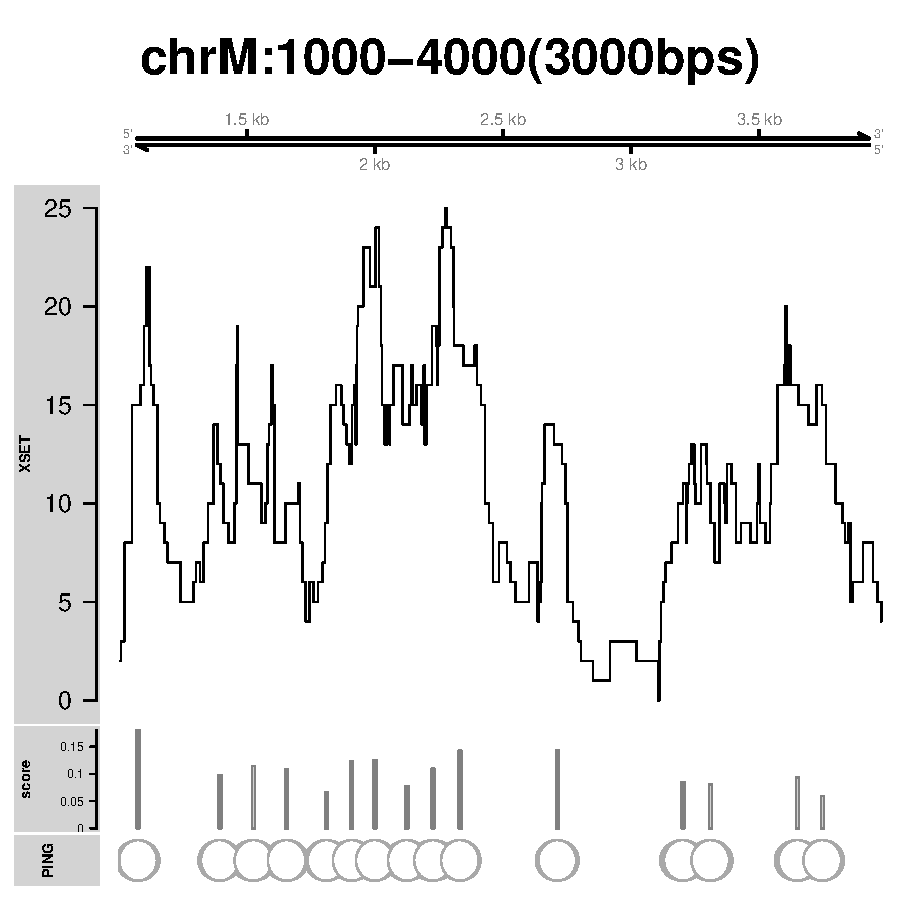
\includegraphics{PING-PE-plotSummary-PE}

%Note that the argument PE should be set to TRUE. 
All the arguments for this function will work for Paired-end data as well. Refer to PING vignette and  the man page ?plotSummary for more information.

\end{document}
